\newcounter{LHCMapLineCounter}
\def\theLHCMapLineCounter{\arabic{LHCMapLineCounter}}
\begin{tikzpicture}
\node[anchor=south west,inner sep=0] at (0,0) {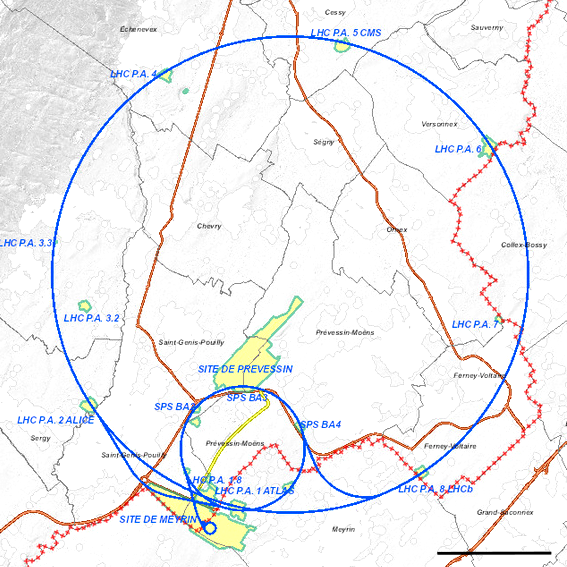
\includegraphics[scale=.35]{\PhDthesisdir/slides/LHC-CMS/LHC/CERN_LHC_map-scale_2km.png}};
\draw (6.125,.4) node {\SI{2}{\kilo\meter}};
\draw (2.95,.75) coordinate (LHCp1);
\draw (1.125,2) coordinate (LHCp2);
\draw (.65,4) coordinate (LHCp3);
\draw (1,3.2) coordinate (LHCp32);
\draw (2,6.1) coordinate (LHCp4);
\draw (4.25,6.45) coordinate (LHCp5);
\draw (6.05,5.15) coordinate (LHCp6);
\draw (6.15,3.125) coordinate (LHCp7);
\draw (5.15,1.15) coordinate (LHCp8);
\draw (LHCp1) coordinate (ATLAS);
\draw (LHCp2) coordinate (ALICE);
\draw (LHCp5) coordinate (CMS);
\draw (LHCp8) coordinate (LHCb);

%\foreach \coord in {1,2,3,4,5,6,7,8,32}{
%\fill[ltcolorred] (LHCp\coord) circle (3pt);
%}

%\draw [ultra thick, ltcolorred] (3.575,3.625) circle (2.95) ;
%\draw [ultra thick, ltcolorred] (3,1.475) circle (.75) ;
%\draw [ultra thick, ltcolorred] (2.6,.5) circle (.075) ;
%\fill [ltcolorred] (2.55,.55) circle (.05) ;
%\draw [ultra thick, ltcolorred] (2.5,.5) --+ (-60:.15) ;

\def\LHCcolor{ltcolorred}
\def\LEPcolor{ltcolorcyan}
\def\RingPtcolor{black}

%\foreach \coord in {1,2,3,4,5,6,7,8,32}{
%\fill[\RingPtcolor] (LHCp\coord) circle (1pt);
%}


\setcounter{LHCMapLineCounter}{0}
\foreach \coord in {DELPHI,L3,OPAL,ALEPH}{
\draw (-.5,{.75+(6.45-.75)*\theLHCMapLineCounter/3}) node (tmp) [left] {\coord};
\draw [ultra thick, \LEPcolor] (tmp.east)--+(.25,0) -- (\coord);
\fill[\LEPcolor] (\coord) circle (4pt);
\stepcounter{LHCMapLineCounter}
}
\setcounter{LHCMapLineCounter}{0}
\foreach \coord in {ATLAS,LHCb,ALICE,CMS}{
\draw (7.5,{.75+(6.45-.75)*\theLHCMapLineCounter/3}) node (tmp) [right] {\coord};
\draw [ultra thick, \LHCcolor] (tmp.west)--+(-.25,0) -- (\coord);
\fill[\LHCcolor] (\coord) circle (4pt);
\stepcounter{LHCMapLineCounter}
}
\foreach \coord in {ALEPH,L3,DELPHI,OPAL}{
\fill[\LEPcolor] (\coord) --+ (110:4pt) arc (110:110+180:4pt);
}

\draw (9,3.6) node {\color{\LHCcolor}\LARGE\bfseries\textsl{LHC}};
\draw (-2,3.6) node {\color{\LEPcolor}\LARGE\bfseries\textsl{LEP}};

\end{tikzpicture}